% !TeX root = ../../thesis.tex

\subsection{\tcs{}}
The second approach closely resembles the previous one. However, instead of permanently removing redundant test cases, \acrfull{tcs} has a notion of context. In this algorithm, we will not calculate the minimal hitting set at runtime, but before executing the test suite, we will perform a \emph{white-box static analysis} of the source code. This analysis identifies which parts of the source code have been changed and executes only the corresponding test cases. Subsequent executions of the test suite will require a new analysis, thus making the selection temporary (\Cref{fig:tcs}) and modification-aware \cite{10.1002/stv.430}. Rothermel and Harrold define this formally in \cref{def:tcs}.

\begin{definition}[\tcs{}]
\label{def:tcs}
\mbox{}\\Given:
\begin{itemize}
	\item $P$ the previous version of the codebase
	\item $P'$ the current (modified) version of the codebase
	\item $T$ the test suite
\end{itemize}

\noindent \tcs{} aims to find a subset $T' \subseteq T$ that is used to test $P'$. 
\end{definition}

\begin{figure}[htbp!]
	\centering
	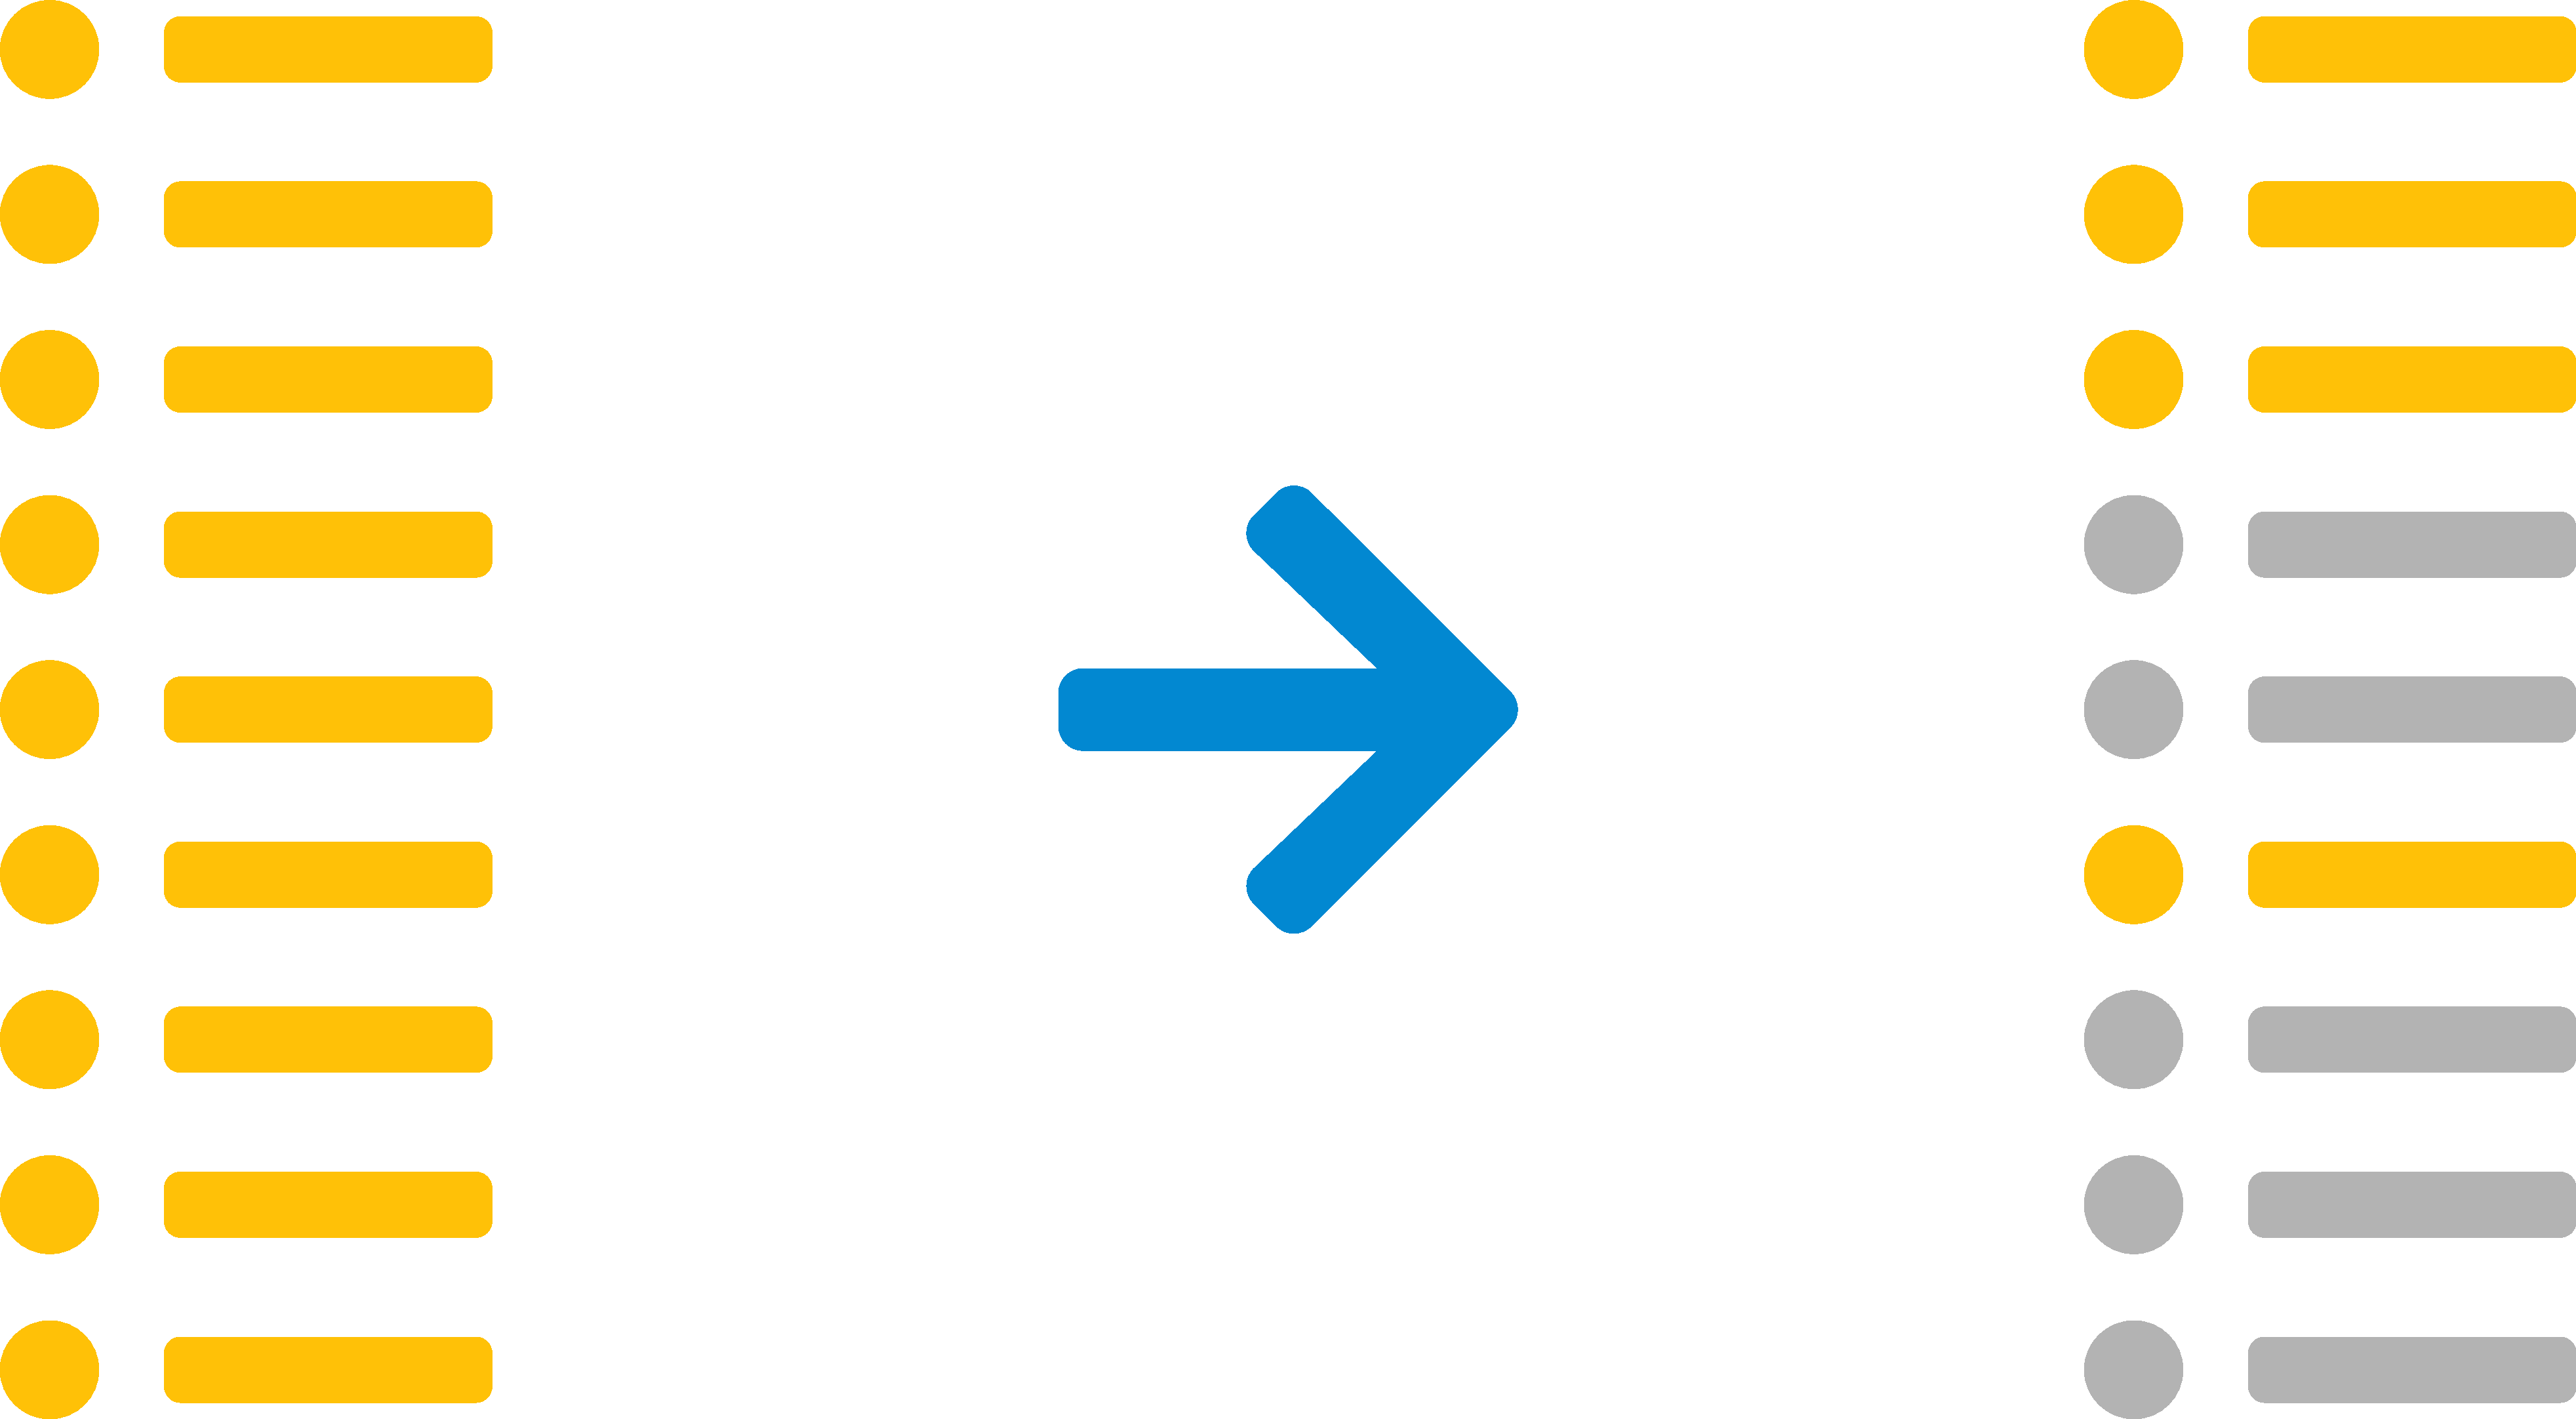
\includegraphics[width=\textwidth]{assets/tikz/approach-tcs.tikz}
	\caption{\tcs{}.}
	\label{fig:tcs}
\end{figure}

\clearpage